\chapter{सरल यंत्र: उत्तोलक, घिरनी, आनत तल}\label{ch:g5:simple-machines}

न इंजन, न बिजली --- फिर भी कुछ शहतीरों, रस्सियों और ढलानों से पुराने
ज़माने के राजगीरों ने ऐसे पत्थर उठा दिए जिन्हें बैलों की पूरी टोलियाँ
भी नहीं घसीट सकती थीं। उनके औज़ार-डिब्बे में \emph{\omterm{def:g5:simple-machines:machine}{सरल यंत्र}} थे:
बिना किसी मोटर वाले वे आविष्कार, जो कमज़ोर और आरामदेह खिंचाव को ताक़तवर
खिंचाव में बदल देते हैं। पहला यंत्र तुम्हारे पास पहले से है; अब पूरे
कुनबे से मिलो।

\section{मेहनत बचाने वालों का कुनबा}

\begin{definition}[सरल यंत्र]\label{def:g5:simple-machines:machine}
\emph{सरल यंत्र}\index{सरल यंत्र} बिना मोटर वाला ऐसा उपकरण है जो \omterm{def:g2:pushes-and-pulls:force}{बल}
को हमारे मन-मुताबिक़ बदल देता है: उसे ताक़तवर बनाकर, या उसकी दिशा
बदलकर, या दोनों करके। पुराने और पक्के सदस्य: सी-सॉ और सब्बल वाला
\emph{\omterm{def:g3:levers-and-scales:lever}{उत्तोलक}} जिसे तुम जानते हो, \emph{\omterm{def:g5:simple-machines:pulley}{घिरनी}}, और
\emph{\omterm{def:g5:simple-machines:ramp}{आनत तल}} --- यानी साधारण-सी ढलान।
\end{definition}

\begin{example}[उत्तोलक, फिर से]\label{ex:g5:simple-machines:lever}
\omterm{def:g3:levers-and-scales:lever}{उत्तोलक} का नियम तुम्हारे पास पहले से है: सिक्के गुणा निशान --- \omterm{def:g3:levers-and-scales:lever}{धुरी}
से दूर लगा तुम्हारा छोटा \omterm{def:g2:pushes-and-pulls:force}{बल} पास रखे बड़े बोझ को मात दे देता है। अब एक
और बात पर ध्यान दो: तुम्हारा सिरा सब्बल के साथ काफ़ी नीचे तक झुकता है
जबकि चट्टान बस ज़रा-सी उठती है। इस \omterm{def:g1:five-senses:observation}{प्रेक्षण} को जेब में सँभाल कर रखो;
वह अभी नियम बनने वाला है।
\end{example}

\section{घिरनियाँ}

\begin{definition}[घिरनी]\label{def:g5:simple-machines:pulley}
\emph{घिरनी}\index{घिरनी} रस्सी के लिए बनी नाली वाला एक पहिया है।
\emph{स्थिर} घिरनी किसी शहतीर से लटकी रहती है और सिर्फ़ खिंचाव की
दिशा बदलती है: नीचे खींचो, बोझ ऊपर जाता है। \emph{चल} घिरनी रस्सी पर
सवार रहती है और बोझ उसी में टँगा होता है: तब बोझ रस्सी की \emph{दो}
लड़ों से लटकता है, और हर लड़ \omterm{def:g4:weight-and-mass:weight}{भार} का सिर्फ़ आधा हिस्सा उठाती है।
\end{definition}

\begin{omfigure}
\begin{tikzpicture}[scale=0.8]
  \draw[thick] (0.2,4.4) -- (2.8,4.4);
  \draw[thick] (1.5,4.4) circle (0.42);
  \draw[thick] (1.08,4.4) -- (1.08,1.6);
  \draw[thick] (1.92,4.4) -- (1.92,2.8);
  \draw[thick, fill=omMeth, fill opacity=0.4]
    (0.68,0.8) rectangle (1.48,1.6);
  \node[font=\footnotesize] at (1.08,1.2) {बोझ};
  \draw[-Stealth, very thick, omThm] (1.92,2.8) -- (1.92,1.9);
  \node[right, font=\small] at (2.1,2.3) {पूरा खिंचाव, नीचे की ओर};
  \node[below, font=\small] at (1.5,0.3) {स्थिर: दिशा बदलती है};
  \begin{scope}[xshift=6.6cm]
    \draw[thick] (0.2,4.4) -- (3.6,4.4);
    \draw[thick] (0.9,4.4) -- (0.9,2.2);
    \draw[thick] (1.74,2.2) circle (0.42) ;
    \draw[thick] (0.9,2.2) arc (180:360:0.42);
    \draw[thick] (2.58,2.2) -- (2.58,4.4);
    \draw[thick] (2.58,3.4) -- (2.58,4.4);
    \draw[thick] (1.74,1.78) -- (1.74,1.5);
    \draw[thick, fill=omMeth, fill opacity=0.4]
      (1.34,0.7) rectangle (2.14,1.5);
    \node[font=\footnotesize] at (1.74,1.1) {बोझ};
    \draw[-Stealth, very thick, omThm] (2.58,4.4) -- (2.58,4.9);
    \node[right, font=\small] at (2.75,4.6) {आधा खिंचाव};
    \node[below, font=\small] at (1.9,0.3)
      {चल: दो लड़ें बोझ बाँट लेती हैं};
  \end{scope}
\end{tikzpicture}

{\small दो घिरनियाँ, दो तोहफ़े। स्थिर \omterm{def:g5:simple-machines:pulley}{घिरनी} तुम्हारे खिंचाव की दिशा
घुमा देती है; चल \omterm{def:g5:simple-machines:pulley}{घिरनी} रस्सी की दो लड़ों को बोझ बाँट लेने देती है,
इसलिए तुम्हारा हाथ सिर्फ़ आधा थामता है।}
\end{omfigure}

\begin{omfigure}
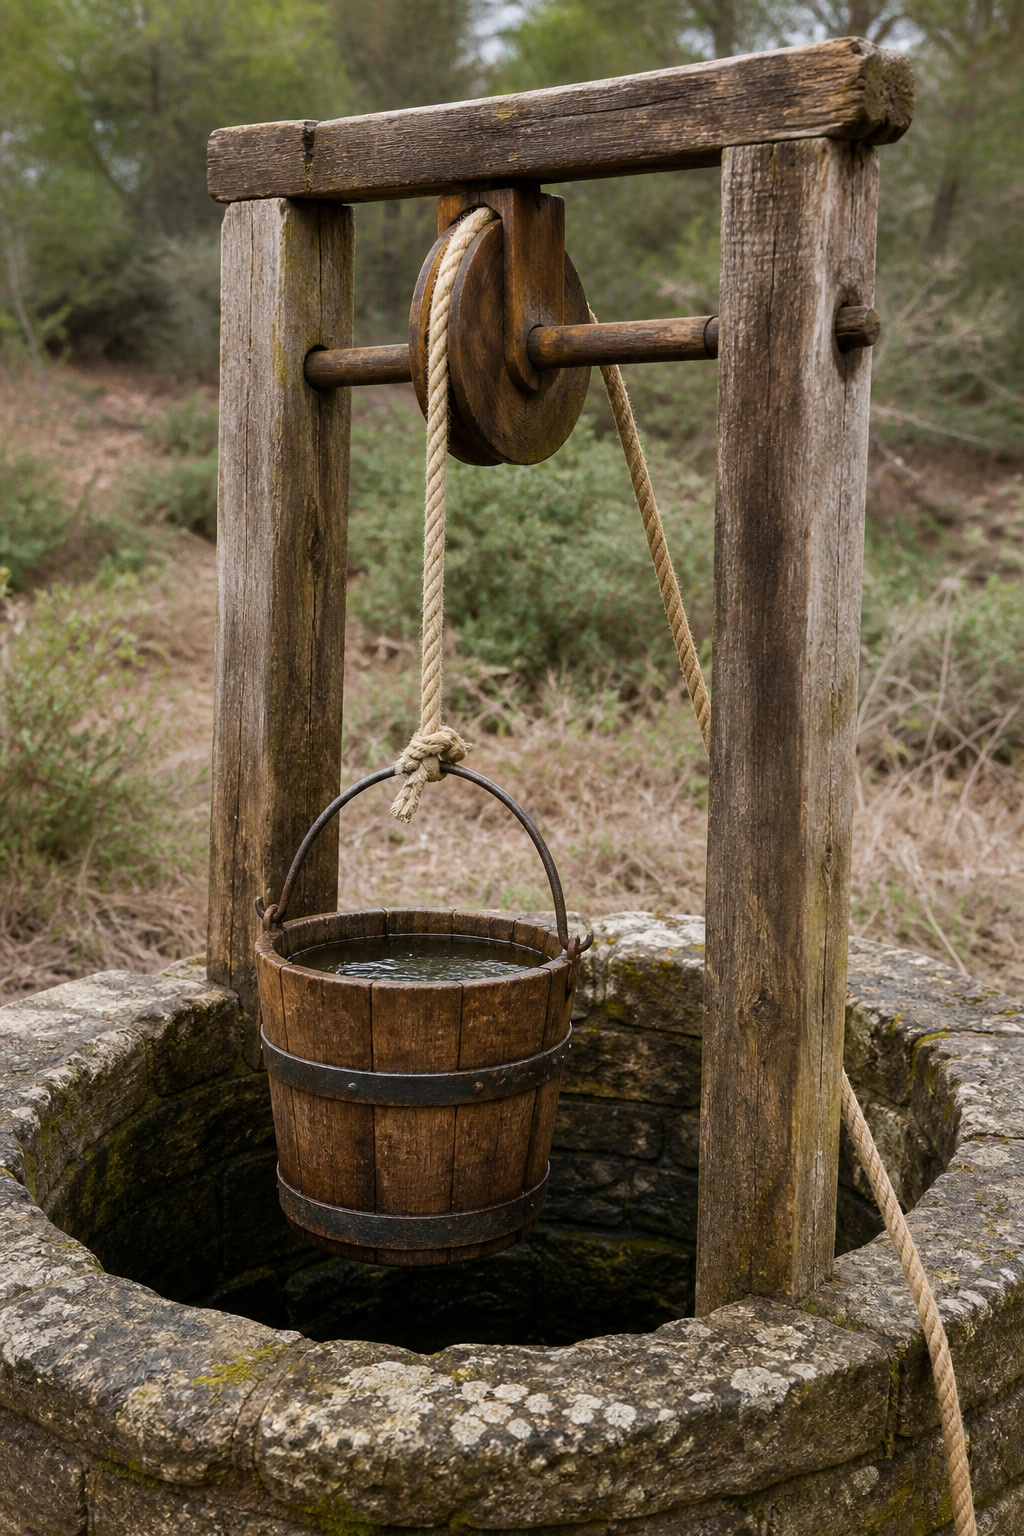
\includegraphics[width=0.34\linewidth]{images/book1/ai/g5-machines-pulley.jpg}

{\small कुएँ की \omterm{def:g5:simple-machines:pulley}{घिरनी}: रस्सी नाली में सवार रहती है, और नीचे की ओर लगा खिंचाव ऊपर उठाने में बदल जाता है।}
\end{omfigure}

\begin{example}[घिरनियाँ काम पर]\label{ex:g5:simple-machines:pulleywork}
झंडा अपने डंडे पर ऊपर चढ़ता जाता है जबकि तुम्हारे हाथ आराम से
\emph{नीचे} की ओर खींचते हैं: ऊपर लगी स्थिर \omterm{def:g5:simple-machines:pulley}{घिरनी} --- दिशा बदली,
मेहनत उतनी ही, पर नीचे खींचने में तुम्हारा अपना \omterm{def:g4:weight-and-mass:weight}{भार} भी मदद करता है।
राजगीरों की घिरनी-मालिका कई घिरनियाँ जोड़ देती है, ताकि बोझ चार या छह
लड़ों से लटके: तब हर लड़ \omterm{def:g4:weight-and-mass:weight}{भार} का चौथाई या छठा हिस्सा उठाती है, और अकेला
मज़दूर पियानो चढ़ा देता है। पर मज़दूर को देखो: उसके हाथों में से
मीटर-दर-मीटर रस्सी दौड़ती जाती है, जबकि पियानो धीरे-धीरे ऊपर सरकता
है।
\end{example}

\section{आनत तल}

\begin{definition}[आनत तल]\label{def:g5:simple-machines:ramp}
\emph{आनत तल}\index{आनत तल} --- यानी ढलान --- बोझ को सीधे ऊपर उठाए
बिना ऊँचाई तक ले जाने का रास्ता है। ढलान जितनी हल्की, बोझ को उस पर
चढ़ाने के लिए उतना ही छोटा धक्का चाहिए: लंबी, हल्की ढलान पर पीपा
लुढ़काना आसान है; छोटी, खड़ी ढलान पर जानलेवा; और सीधे ऊपर, नामुमकिन।
\end{definition}

\begin{method}[रबर बैंड की तुला से इसे महसूस करो]\label{met:g5:simple-machines:measure}
पिछले साल वाली तुम्हारी रबर बैंड की \omterm{def:g3:levers-and-scales:scale}{तुला} यह फ़र्क़ चख सकती है:
\begin{enumerate}
  \item एक पटरे पर खिलौना गाड़ी रखो और उससे रबर बैंड बाँध दो;
  \item पटरे को किताबों के नीचे ढेर पर टिकाकर हल्की ढलान बनाओ; बैंड
        से गाड़ी को धीरे-धीरे ऊपर खींचो और फैलाव नोट करो;
  \item अब उसी पटरे को कुर्सी की गद्दी पर टिकाकर कहीं ज़्यादा खड़ा
        करो, और फिर खींचो।
\end{enumerate}
खड़ी ढलान पर खींचने से बैंड कहीं ज़्यादा फैलता है: ढलान जितनी खड़ी,
मेहनत उतनी बड़ी। हल्की ढलानें सचमुच हल्की होती हैं --- तुम्हारा उपकरण
यही कहता है।
\end{method}

\begin{omfigure}
\begin{tikzpicture}[scale=0.8]
  \draw[thick] (0,0) -- (11.2,0);
  \draw[very thick, omDef] (0.3,0) -- (6.5,2.0);
  \draw[thick, fill=omMeth, fill opacity=0.4]
    (2.8,0.82) rectangle ++(0.8,0.55);
  \draw[-Stealth, thick, omThm] (3.75,1.35) -- (4.65,1.64);
  \node[above, font=\small, omThm] at (3.4,1.75) {छोटा धक्का};
  \draw[very thick, omDef] (8.2,0) -- (10.2,2.0);
  \draw[thick, fill=omMeth, fill opacity=0.4]
    (8.75,0.5) rectangle ++(0.8,0.55);
  \draw[-Stealth, very thick, omThm] (9.75,1.25) -- (10.55,2.05);
  \node[above, font=\small, omThm] at (9.3,1.9) {बड़ा धक्का};
  \node[below, font=\small] at (3.4,-0.3)
    {उसी ऊँचाई तक लंबी हल्की ढलान};
  \node[below, font=\small] at (9.3,-0.3) {छोटी खड़ी ढलान};
\end{tikzpicture}

{\small वही पेटी, वही ऊँचाई पानी है: लंबी हल्की ढलान लंबी सड़क पर
छोटा धक्का माँगती है; खड़ी ढलान छोटी सड़क पर बड़ा धक्का।}
\end{omfigure}

\begin{example}[इलाक़े में ढलानें]\label{ex:g5:simple-machines:ramps}
पहियेदार कुर्सी की ढलानें छोटी सीढ़ियों के बग़ल में लंबी और हल्की
बनाई जाती हैं --- हल्कापन जान-बूझकर रखा जाता है। पहाड़ी सड़कें
टेढ़ी-मेढ़ी घूमती हैं: चोटी पर सीधे चढ़ाई करने के बजाय वे ढलान पर
आगे-पीछे \omterm{def:g2:pushes-and-pulls:force}{बल} खाती एक लंबी, हल्की \omterm{def:g5:simple-machines:ramp}{आनत तल} बिछा देती हैं। और पेच तो
भेस बदले हुए ढलान ही है --- एक छड़ के चारों ओर लिपटी ढलान, जिससे
पेचकस का हर आसान घुमाव पेच को चुपके से एक नन्हा क़दम और गहरा ले जाता
है।
\end{example}

\section{सुनहरा नियम}

\begin{proposition}[यंत्रों का सुनहरा नियम]\label{prop:g5:simple-machines:golden}
कोई \omterm{def:g5:simple-machines:machine}{सरल यंत्र} मुफ़्त में कुछ नहीं देता: वह \omterm{def:g2:pushes-and-pulls:force}{बल} में जितना बचाता है,
दूरी में उतना ही वसूल लेता है। आधा \omterm{def:g2:pushes-and-pulls:force}{बल} --- तो दोगुनी रस्सी खींचनी
पड़ेगी, या दोगुनी सड़क चलनी पड़ेगी; दसवाँ हिस्सा \omterm{def:g2:pushes-and-pulls:force}{बल} --- तो दस गुनी
सड़क। यंत्र-दर-यंत्र यह सौदा ठीक-ठीक बराबर रहता है: आराम मीटरों से
ख़रीदा जाता है।
\end{proposition}

\begin{example}[नियम की जाँच]\label{ex:g5:simple-machines:check}
चल \omterm{def:g5:simple-machines:pulley}{घिरनी}: तुम्हारा हाथ आधे \omterm{def:g2:pushes-and-pulls:force}{बल} से खींचता है, और बोझ को \qty{1}{m}
ऊपर उठाने के लिए तुम्हें \qty{2}{m} रस्सी खींचनी पड़ती है --- दोनों
लड़ों को एक-एक \omterm{def:g2:measuring-length:units}{मीटर} छोटा होना ही है। सब्बल: तुम्हारा सिरा लंबी चाप
में झुकता है, और चट्टान बमुश्किल हिलती है। ढलान: पेटी उसी ऊँचाई तक
पहुँच जाती है, पर तुमने उसे पूरी ढलान भर धकेला है। हर बचत का दाम
चुकाया गया, वह भी ठीक-ठीक।
\end{example}

\begin{remark}[सुनहरे नियम में धोखाधड़ी क्यों नहीं चलती]\label{rem:g5:simple-machines:whygolden}
सुनहरे नियम के नीचे \omterm{def:g5:everyday-energy:energy}{ऊर्जा} वाले अध्याय का हमारा पुराना दोस्त छिपा है:
किसी बोझ को किसी ऊँचाई तक उठाने की एक तय क़ीमत \omterm{def:g5:everyday-energy:energy}{ऊर्जा} में होती है, और
रस्सियों तथा पटरों की कोई भी जमावट उस दाम को नहीं बदलती। यंत्र बस
इतना करते हैं कि तुम्हें वही दाम छोटे सिक्कों में चुकाने देते हैं ---
बस सिक्के ज़्यादा। लंबी सड़क पर छोटा \omterm{def:g2:pushes-and-pulls:force}{बल} उतनी ही \omterm{def:g5:everyday-energy:energy}{ऊर्जा} सौंपता है जितनी
छोटी सड़क पर बड़ा \omterm{def:g2:pushes-and-pulls:force}{बल}। हमेशा चलने वाली मशीनें ठीक इसी वजह से नाकाम
रहीं: बिल आख़िर बिल ही होता है।
\end{remark}

\section{अभ्यास}

\begin{exercise}[$\star$]\label{exo:g5:simple-machines:1}
तीनों पुराने सरल यंत्रों के नाम बताओ, और हर एक की एक रोज़मर्रा की
जगह।
\end{exercise}

\begin{exercise}[$\star$]\label{exo:g5:simple-machines:2}
स्थिर \omterm{def:g5:simple-machines:pulley}{घिरनी} तुम्हारे खिंचाव में क्या बदलती है? और चल \omterm{def:g5:simple-machines:pulley}{घिरनी} क्या
बदलती है?
\end{exercise}

\begin{exercise}[$\star$]\label{exo:g5:simple-machines:3}
झंडा चढ़ाने के लिए रस्सी \emph{नीचे} की ओर खींचना उसी \omterm{def:g4:weight-and-mass:weight}{भार} को सीधे
ऊपर उठाने से ज़्यादा आरामदेह क्यों है, जबकि मेहनत उतनी ही होती है?
\end{exercise}

\begin{exercise}[$\star$]\label{exo:g5:simple-machines:4}
एक चल \omterm{def:g5:simple-machines:pulley}{घिरनी} के साथ बोझ दो लड़ों से लटकता है। तुम्हारा हाथ \omterm{def:g4:weight-and-mass:weight}{भार} का
कितना हिस्सा थामता है? बोझ को \qty{3}{m} ऊपर उठाने के लिए कितनी
रस्सी खींचनी पड़ेगी?
\end{exercise}

\begin{exercise}[$\star$]\label{exo:g5:simple-machines:5}
\cref{met:g5:simple-machines:measure} में कौन-सी ढलान रबर बैंड को
ज़्यादा फैलाती है? हल्की ढलान के छोटे फैलाव का दाम क्या चुकाता है?
\end{exercise}

\begin{exercise}[$\star$]\label{exo:g5:simple-machines:6}
पहाड़ी सड़कें सीधे ऊपर चढ़ने के बजाय टेढ़ी-मेढ़ी क्यों घूमती हैं?
पूरी सड़क कौन-सा \omterm{def:g5:simple-machines:machine}{सरल यंत्र} है?
\end{exercise}

\begin{exercise}[$\star$]\label{exo:g5:simple-machines:7}
यंत्रों का सुनहरा नियम बताओ। कोई यंत्र तुम्हें दसवें हिस्से \omterm{def:g2:pushes-and-pulls:force}{बल} से
खींचने देता है --- वह तुमसे क्या वसूलता है?
\end{exercise}

\begin{exercise}[$\star$]\label{exo:g5:simple-machines:8}
पेच भेस बदला हुआ \omterm{def:g5:simple-machines:ramp}{आनत तल} कैसे है? उसमें लंबी हल्की सड़क की भूमिका कौन
निभाता है?
\end{exercise}

\begin{exercise}[$\star\star$]\label{exo:g5:simple-machines:9}
एक घिरनी-मालिका पियानो को चार लड़ों से लटकाती है। मज़दूर का हाथ
पियानो के \omterm{def:g4:weight-and-mass:weight}{भार} का कौन-सा भाग खींचता है? पियानो को \qty{2}{m} ऊपर
उठाने के लिए उसके हाथों में से कितने \omterm{def:g2:measuring-length:units}{मीटर} रस्सी गुज़रेगी?
\end{exercise}

\begin{exercise}[$\star\star$]\label{exo:g5:simple-machines:10}
सामान चढ़ाने की एक ढलान \qty{6}{m} लंबी है और \qty{1}{m} ऊपर उठती
है; उस पर पेटी धकेलने में हल्का-सा ज़ोर लगता है। जल्दबाज़ मज़दूर उसी
चबूतरे तक सिर्फ़ \qty{3}{m} लंबी नई ढलान बना लेते हैं। सुनहरे नियम
से नए और पुराने धक्के की तुलना करो --- और बताओ कि ``आधी सड़क'' कोई
सस्ता सौदा क्यों नहीं था।
\end{exercise}

\begin{exercise}[$\star\star$]\label{exo:g5:simple-machines:11}
एक विज्ञापन ऐसी घिरनी-मालिका बेचता है जो ``इतनी चतुर है कि तुम आधे
\omterm{def:g2:pushes-and-pulls:force}{बल} से एक \omterm{def:g2:measuring-length:units}{मीटर} रस्सी खींचते हो --- और बोझ पूरा एक \omterm{def:g2:measuring-length:units}{मीटर} ऊपर उठ जाता
है''। इस दावे को सुनहरे नियम और
\cref{rem:g5:simple-machines:whygolden} के ऊर्जा-बिल के सामने कठघरे
में खड़ा करो: क्या पहियों और रस्सियों की कोई भी जमावट इसे निभा सकती
है?
\end{exercise}
